\documentclass{article}
\usepackage{graphicx}
\usepackage{amsmath}

\begin{document}

\title{Problem 17 - Arctangent function by numerical root finding}
\author{Jens S. K. Jensen}
\date{\today}
\maketitle

\section{Introduction}
This report 

\section{Plot visualization}


\begin{figure}
	\centering
	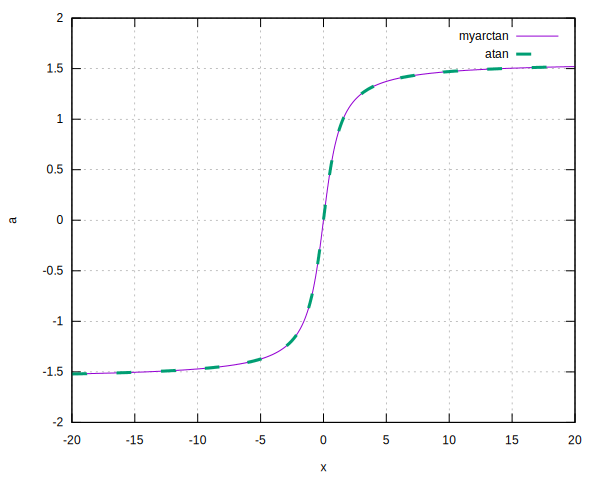
\includegraphics{plot.pdf}
	\caption{Visualization of the arctan function, showing both own numerical (myarctan) and the atan definition from math.h}
	\label{fig:plot}
\end{figure}

\end{document}
